\documentclass[a4paper,10pt]{ctexart}
\usepackage[margin=1in]{geometry}

%\usepackage{aicescover} %使用新的封面

%\usepackage{titletoc} %使用此包目录生成Bug
\usepackage{abstract}
\usepackage{graphics}
\usepackage{amsmath}
\usepackage{amsfonts}
\usepackage{amssymb}
\usepackage{amsthm}

\usepackage{cite}

\usepackage[colorlinks,linkcolor=black,anchorcolor=blue,citecolor=green]{hyperref}

\usepackage{clrscode3e} %插入伪代码

\usepackage{listings} %插入C代码
\usepackage{xcolor}
\lstset{
    %行号
    numbers=left,
    %背景框
    framexleftmargin=10mm,
    frame=none,
    %背景色
    %backgroundcolor=\color[rgb]{1,1,0.76},
    backgroundcolor=\color[RGB]{245,245,244},
    %样式
    keywordstyle=\bf\color{blue},
    identifierstyle=\bf,
    numberstyle=\color[RGB]{0,192,192},
    commentstyle=\it\color[RGB]{0,96,96},
    stringstyle=\rmfamily\slshape\color[RGB]{128,0,0},
    %显示空格
    showstringspaces=false
}

\ctexset{section={
    name={第,章},
    number=\arabic{section},
    }
}

\begin{document}
%\maketitle
\begin{titlepage}

\begin{center}


% Upper part of the page

\includegraphics[width=0.8\textwidth]{../Pics/HIT.eps}\\[1cm]

\textsc{\LARGE Harbin Institute of Technology}\\[1.5cm]

% Title
\hrulefill \\[0.4cm]
{ \huge \bfseries 集合论实验报告:最小生成树}\\[0.4cm]
\hrulefill \\[1.5cm]

% Author and supervisor
\begin{minipage}{0.4\textwidth}
\begin{flushleft} \large
%悬空
\end{flushleft}
\end{minipage}
\begin{minipage}{0.4\textwidth}
\begin{flushright} \large
\emph{作者:}冯云龙 \\
\emph{学号:}1160300202
\end{flushright}
\end{minipage}

\vfill

% Bottom of the page
{\large \today}

\end{center}
\end{titlepage}

\part*{摘要}
生活中的许许多多看似不同的问题在本质上却是相同的,我们往往会遇到求整体最短、最近、最省钱的问题...这个时候,通过对图论问题的研究,我们就可以对这些问题做出解答,此报告主要回答关于图论中最小生成树的问题。
paragraph{关键词:}$Prim$\ \ $Kruskal$\ \ 最小生成树
\tableofcontents

\newpage
\part{正文}
\section{实验背景}

\subsection{实验目的}
\paragraph{实际问题} 我们常常会遇到求整体最短、最近、最省钱这些方面的问题,就比如下列问题:
\begin{itemize}
\item 镇子里要铺设自来水管道,怎么铺用的水管最少,而且家家都能用到水。
\item 在电路设计中,常常需要把一些电子元件的插脚用电线连接起来。 如果每根电线连接两个插脚,把所有n个插脚连接起来,只要用n-1根电线就可以了。 在所有的连接方案中,我们通常对电线总长度最小的连接方案感兴趣。
\item 要在n个城市之间铺设光缆,主要目标是要使这 n 个城市的任意两个之间都可以通信, 找出一条使用最短的光纤连通这些城市的铺设方法。
\end{itemize}
而像这样的问题,我们都可以通过将其转化为图的问题来解决。

\subsection{实验方法}
诸如以上问题,我们都可以通过将其转化成图,而后使用求解图的方法解决它。
例如,上述一个铺设管道的问题,我们就可以将其按如下方式转化:
取图$G(V,E,W)$,城镇所对应的顶点集$(V_0,V_1...V_{n-1}) \in V $,若两个城镇$V_i,V_j$邻接,距离为$w$,则有$(V_i,V_j)\in E$,$W(V_i,V_j)=w$。

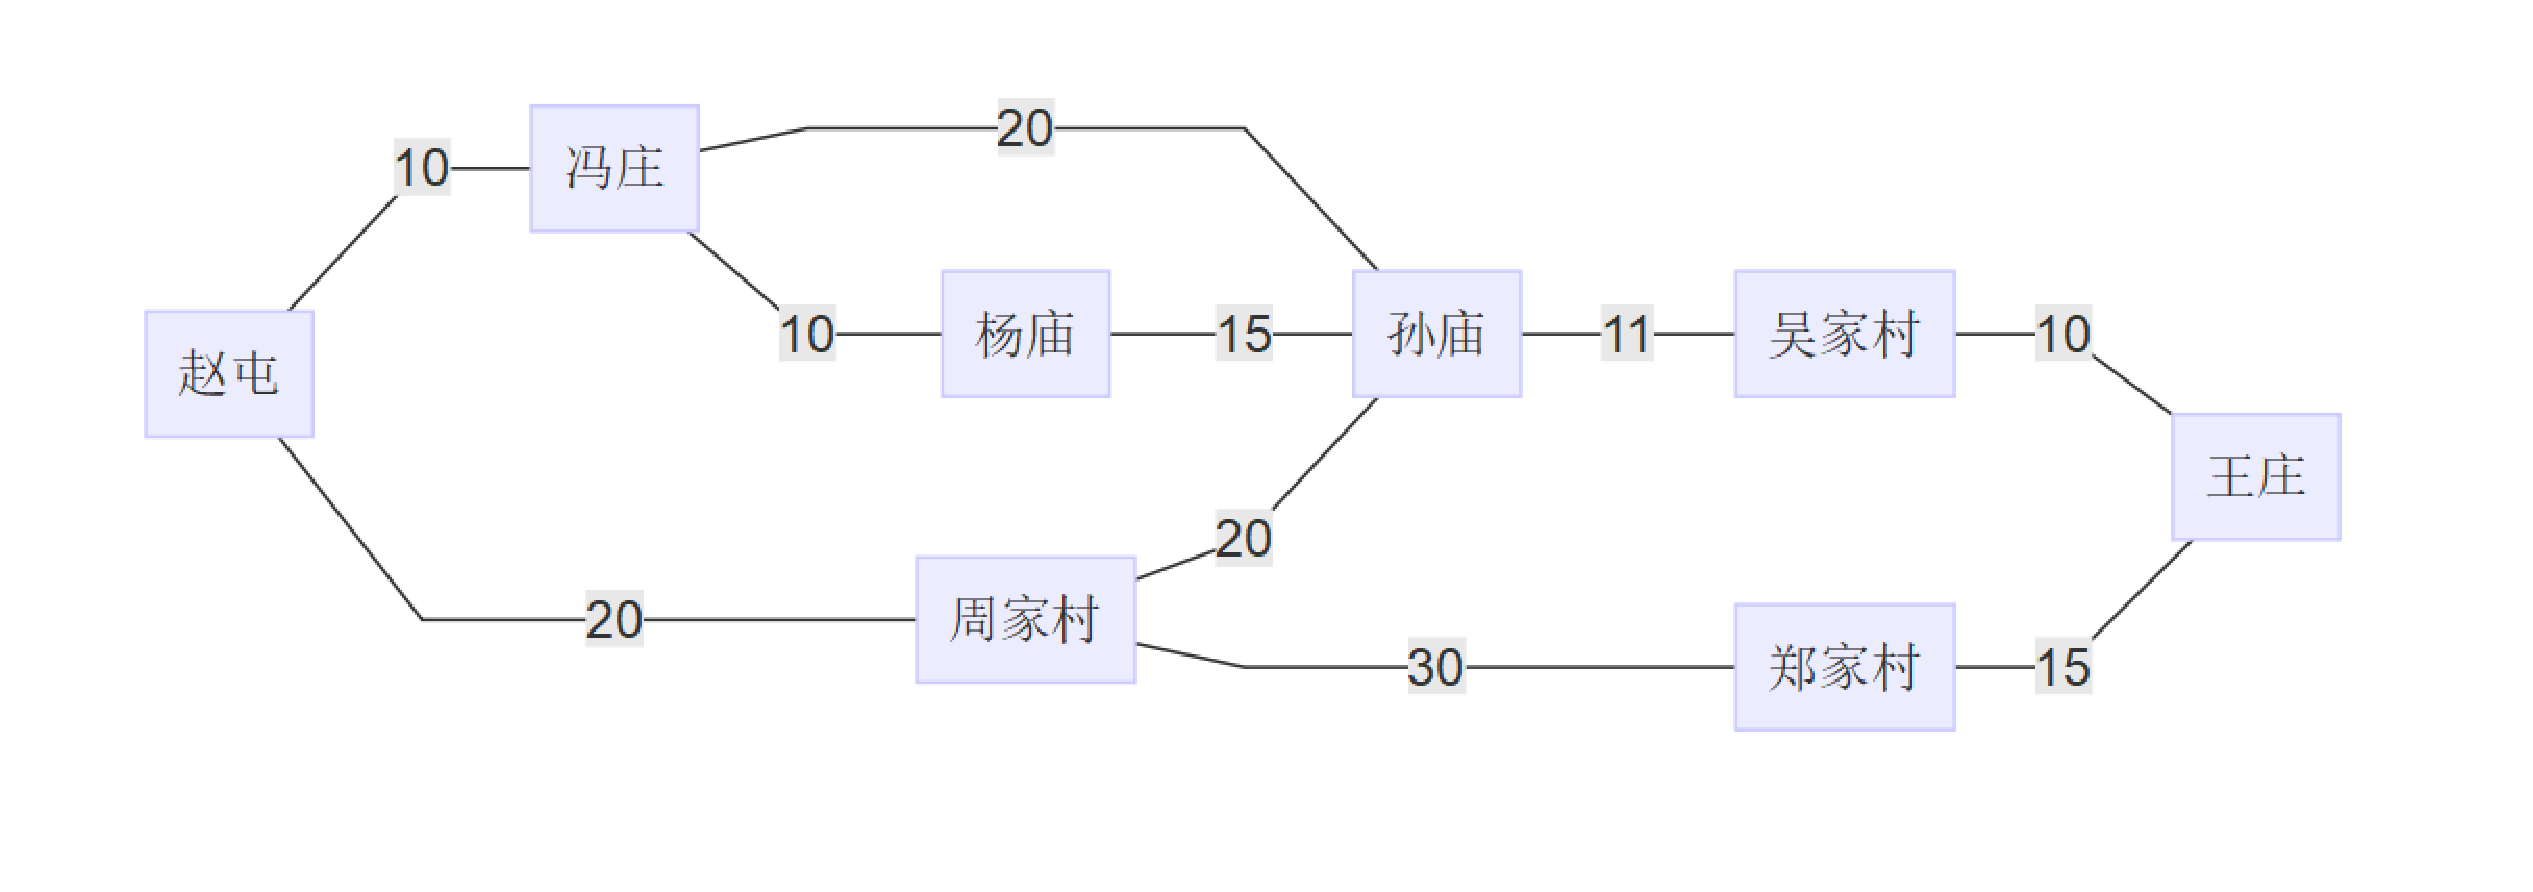
\includegraphics[width=0.9\textwidth]{../Pics/MiniTree.eps}

\section{实验原理}
\subsection{$Prim$算法}
\subsubsection{介绍}
\paragraph{普里姆算法($Prim$算法)}
图论中的一种算法,可在加权连通图里搜索最小生成树。\\
该算法于1930年由捷克数学家沃伊捷赫·亚尔尼克(英语:Vojtěch Jarník)发现;
并在1957年由美国计算机科学家罗伯特·普里姆(英语:Robert C. Prim)独立发现;
1959年,艾兹格·迪科斯彻再次发现了该算法。\\
因此,在某些场合,普里姆算法又被称为DJP算法、亚尔尼克算法或普里姆-亚尔尼克算法。

\subsubsection{算法步骤}
\begin{enumerate}
  \item 获得$G(V,E,W)$,新建图$G_{new}(V_{new},E_{new},W_{new})$。
  \item 初始化:$V_{new} = \{x\}$,
        其中x为集合V中的任一节点(起始点),
        $E_{new} = \{ \} $;
  \item 重复下列操作,直到$V_{new} = V$:
    \begin{enumerate}
        \item 在集合$E$中选取权值最小的边$<u, v>$,
        其中$u\in V_{new},v \not\in V_ {new}$(如果存在有多条满足前述条件即具有相同权值的边,则可任意选取其中之一)。
        \item   将$v$加入集合$V_{new}$中,
                将$<u,v>$边加入集合$E_{new}$中,
                将$W<u,v>$加入到$W_{new}$。
  \end{enumerate}
  \item 输出:$G_{new}(V_{new},E_{new},W_{new})$。
\end{enumerate}

\subsection{$Kruskal$算法}
\subsubsection{介绍}
\paragraph{$Kruskal$算法}是一种用来寻找最小生成树的算法,由Joseph Kruskal在1956年发表。
用来解决同样问题的还有Prim算法和Boruvka算法等。
三种算法都是贪婪算法的应用。
和Boruvka算法不同的地方是,Kruskal算法在图中存在相同权值的边时也有效。
\subsubsection{算法步骤}
\begin{enumerate}
  \item 获得$G(V,E,W)$,新建图$G_{new}(V_{new},E_{new},W_{new})$,使$V_{new} = V$。
  \item 将原图$G(V,E,W)$中所有边按权值从小到大排序。
  \item 重复以下操作,直至图$G_{new}$中所有的节点都在同一个连通分量中。
      \begin{enumerate}
       \item 获取$G$中的权值最小的边(若获取过则不再获取)。
       \item 如果这条边连接的两个节点于图$G_{new}$中且不在同一个连通分量中,则添加这条边到图$G_{new}$中。
      \end{enumerate}
  \item 输出:$G_{new}(V_{new},E_{new},W_{new})$。
\end{enumerate}


\section{代码实现}
\subsection{设计数据结构}
参照了耶鲁大学的一位前辈的代码,动态分配数组,长度可以扩展,既不浪费空间,又不会带来性能损失。
数据结构如下:

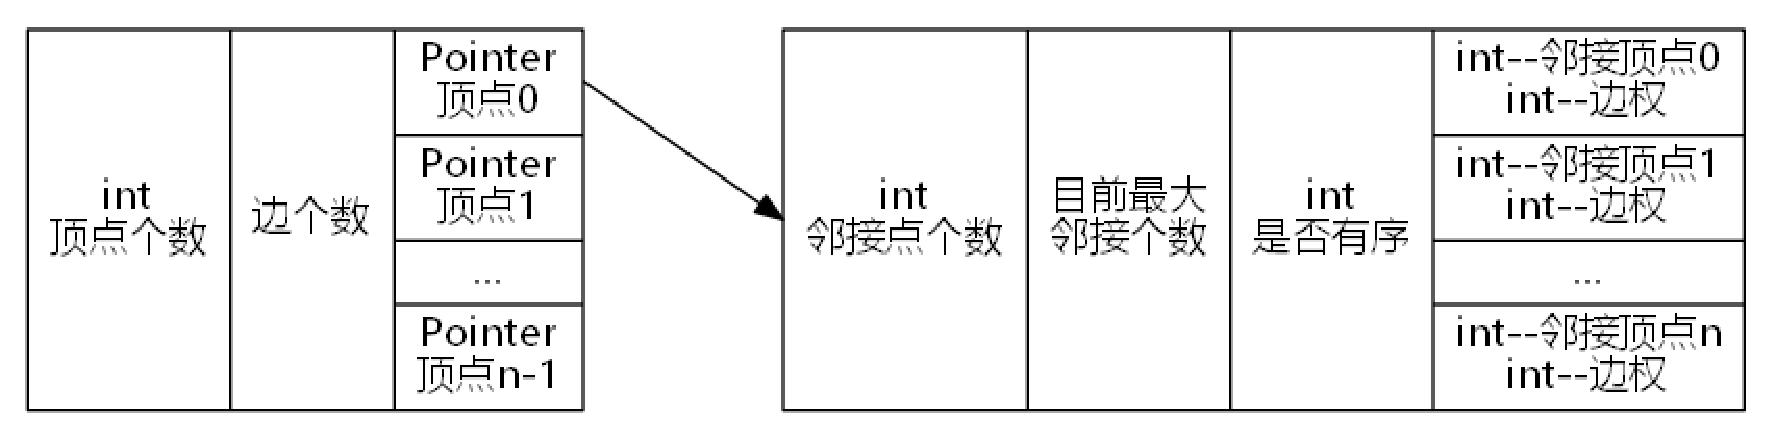
\includegraphics[width=0.9\textwidth]{../Pics/DataStruct.eps}

\newpage
结构代码实现如下:
\begin{lstlisting}[language={C}]

typedef struct _list {
    int vec;                    //临接顶点
    int weight;                 //权
} link_list;

struct w_graph {
    int n;                      //顶点个数
    int m;                      //边个数
    struct successors {
        int d;                  //临接点个数
        int len;                //最大临接点个数
        char is_sorted;         //是否有序
        link_list list[1];      //临接列表
    } *v_list[1];               //注意:这是一个指针的数组
};

typedef struct w_graph *WGraph;//图是一个指针类型的
\end{lstlisting}
\subsection{设计数据操作}

\paragraph{创建一个顶点从$0 \to n-1$的带权图}分配初始内存,此时分配内存时多分配$n-1$块$Struct\ Succesors^*$(顶点的邻接列表指针)大小的地址,并对每个指针分配默认大小的内存。
\paragraph{从内存中删去一个图}遍历释放各顶点邻接列表的内存,再释放图的内存。
\paragraph{添加边和权}首先确定是否需要对邻接列表的内存进行扩展(使用指数递增的策略扩展),使用$relloc$函数对已经分配的内存进行改变,此时实际上对$link\_list$数组进行了扩容。
\paragraph{返回顶点个数}返回n。
\paragraph{返回边个数}返回m。
\paragraph{返回顶点的度}返回$v\_list[V].d$。
\paragraph{判断是否邻接}通过该点度的大小来确定是否需要对邻接列表排序,数据量少的时候进行遍历。
\paragraph{获取边的权}通过该点度的大小来确定是否需要对邻接列表排序,数据量少的时候进行遍历,而后返回权值。
\paragraph{提供读取顶点数据的接口}接受函数指针$Func$和所需数据指针,内部对邻接列表里的每个顶点施加$Func$操作(将原点,邻接点和权都传给该函数以供操作)。

\subsection{实现最小生成树算法}
\begin{itemize}
\item $Prim$算法实现(伪代码)
\begin{codebox}
\Procname{$\proc{Prim Algorithm}(G,v_0)$}
\li $v_{new} = v_0,G_{new}(V_{new},E_{new},W_{new})$
\li \While $V_{new} \ne V$
    \Do
\li     $Get\ u\in V_{new},v\not\in V_{new}\ Make\ W(u,v)\ min$
\li     $Set\ v \in V_{new}$,\ $Set\ <u,v>\in E_{new}$,\ $Set\ W(u,v)\in W_{new}$
    \End
\end{codebox}
\item $Kruskal$算法实现(伪代码)
堆的实现在Github上,此处不再赘述。
\begin{codebox}
\Procname{$\proc{Prim Algorithm}(G)$}
\li $G_{new}(V_{new},E_{new},W_{new}),V_{new}=V$
\li $Sort\ W$
\li $Set \  v_0 \in S$
\li \While $\exists u,v \in V_{new},Set_u \not= Set_v$
    \Do
\li     $<u,v> \gets \attrib{Dis(W)}{Min}$
\li     \If $Set_u \not= Set_v$
        \Do
\li        $Set \ W(u,v) \in W_{new}$
\li        $Merge\ (Set_u,Set_v)$
        \End
    \End
\end{codebox}
\end{itemize}

\section{实验结果}
\subsection{数据输入}
输入如下无向带权图\\
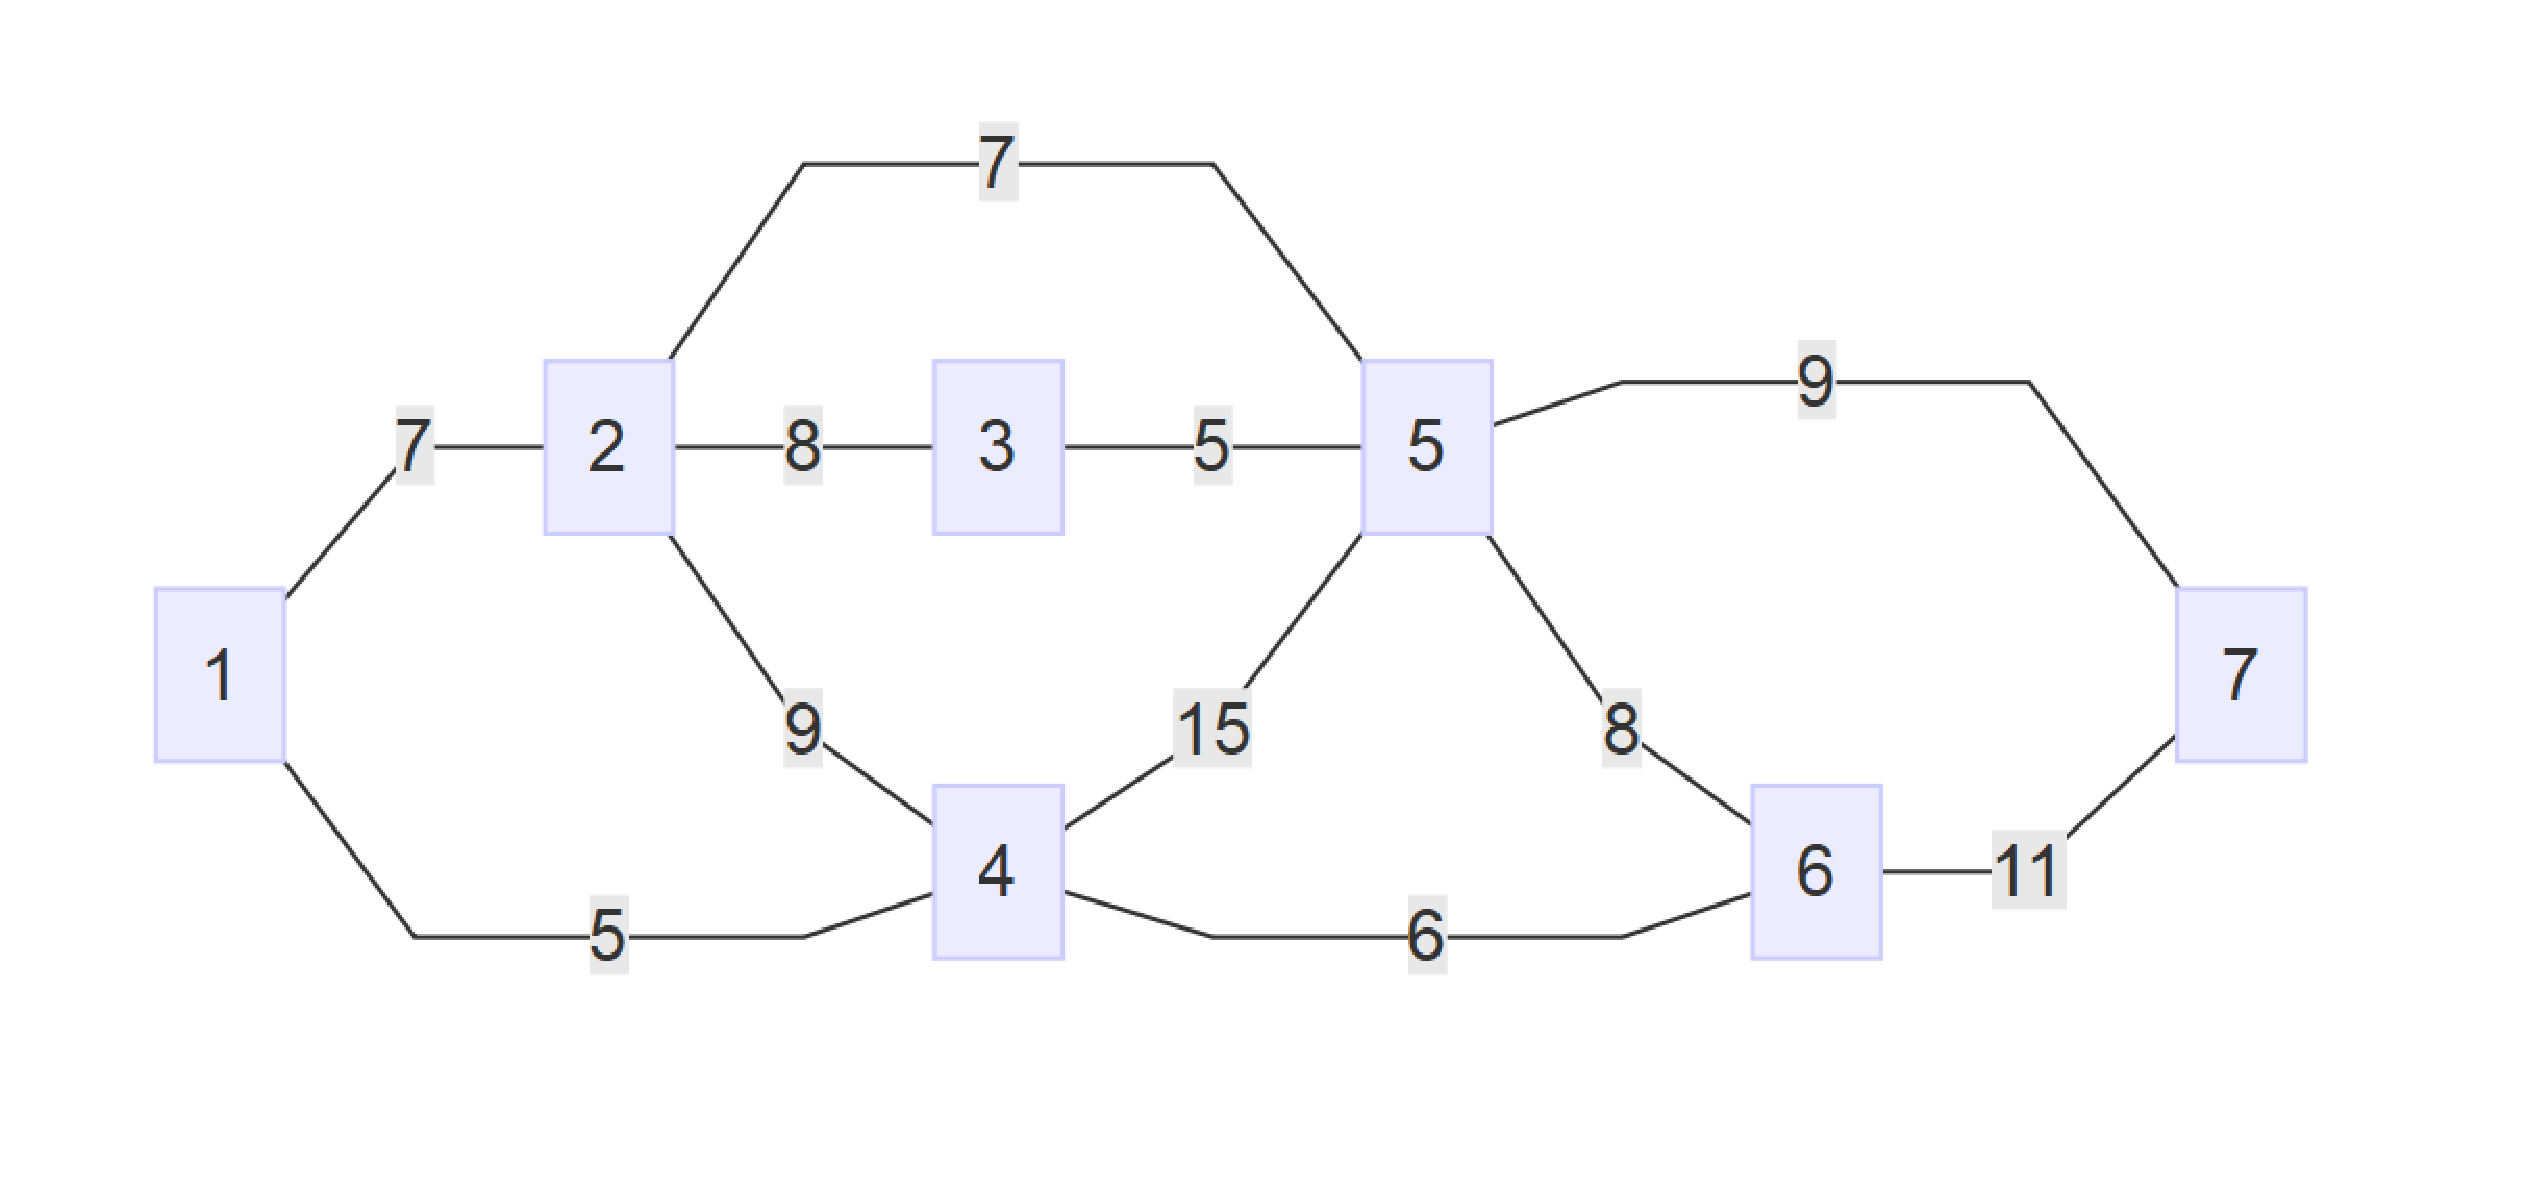
\includegraphics[width=0.9\textwidth]{../Pics/Test-MiniTree.eps}
\subsection{结果输出}
通过$Prim$算法或$Kruskal$算法可得到如下结果\\
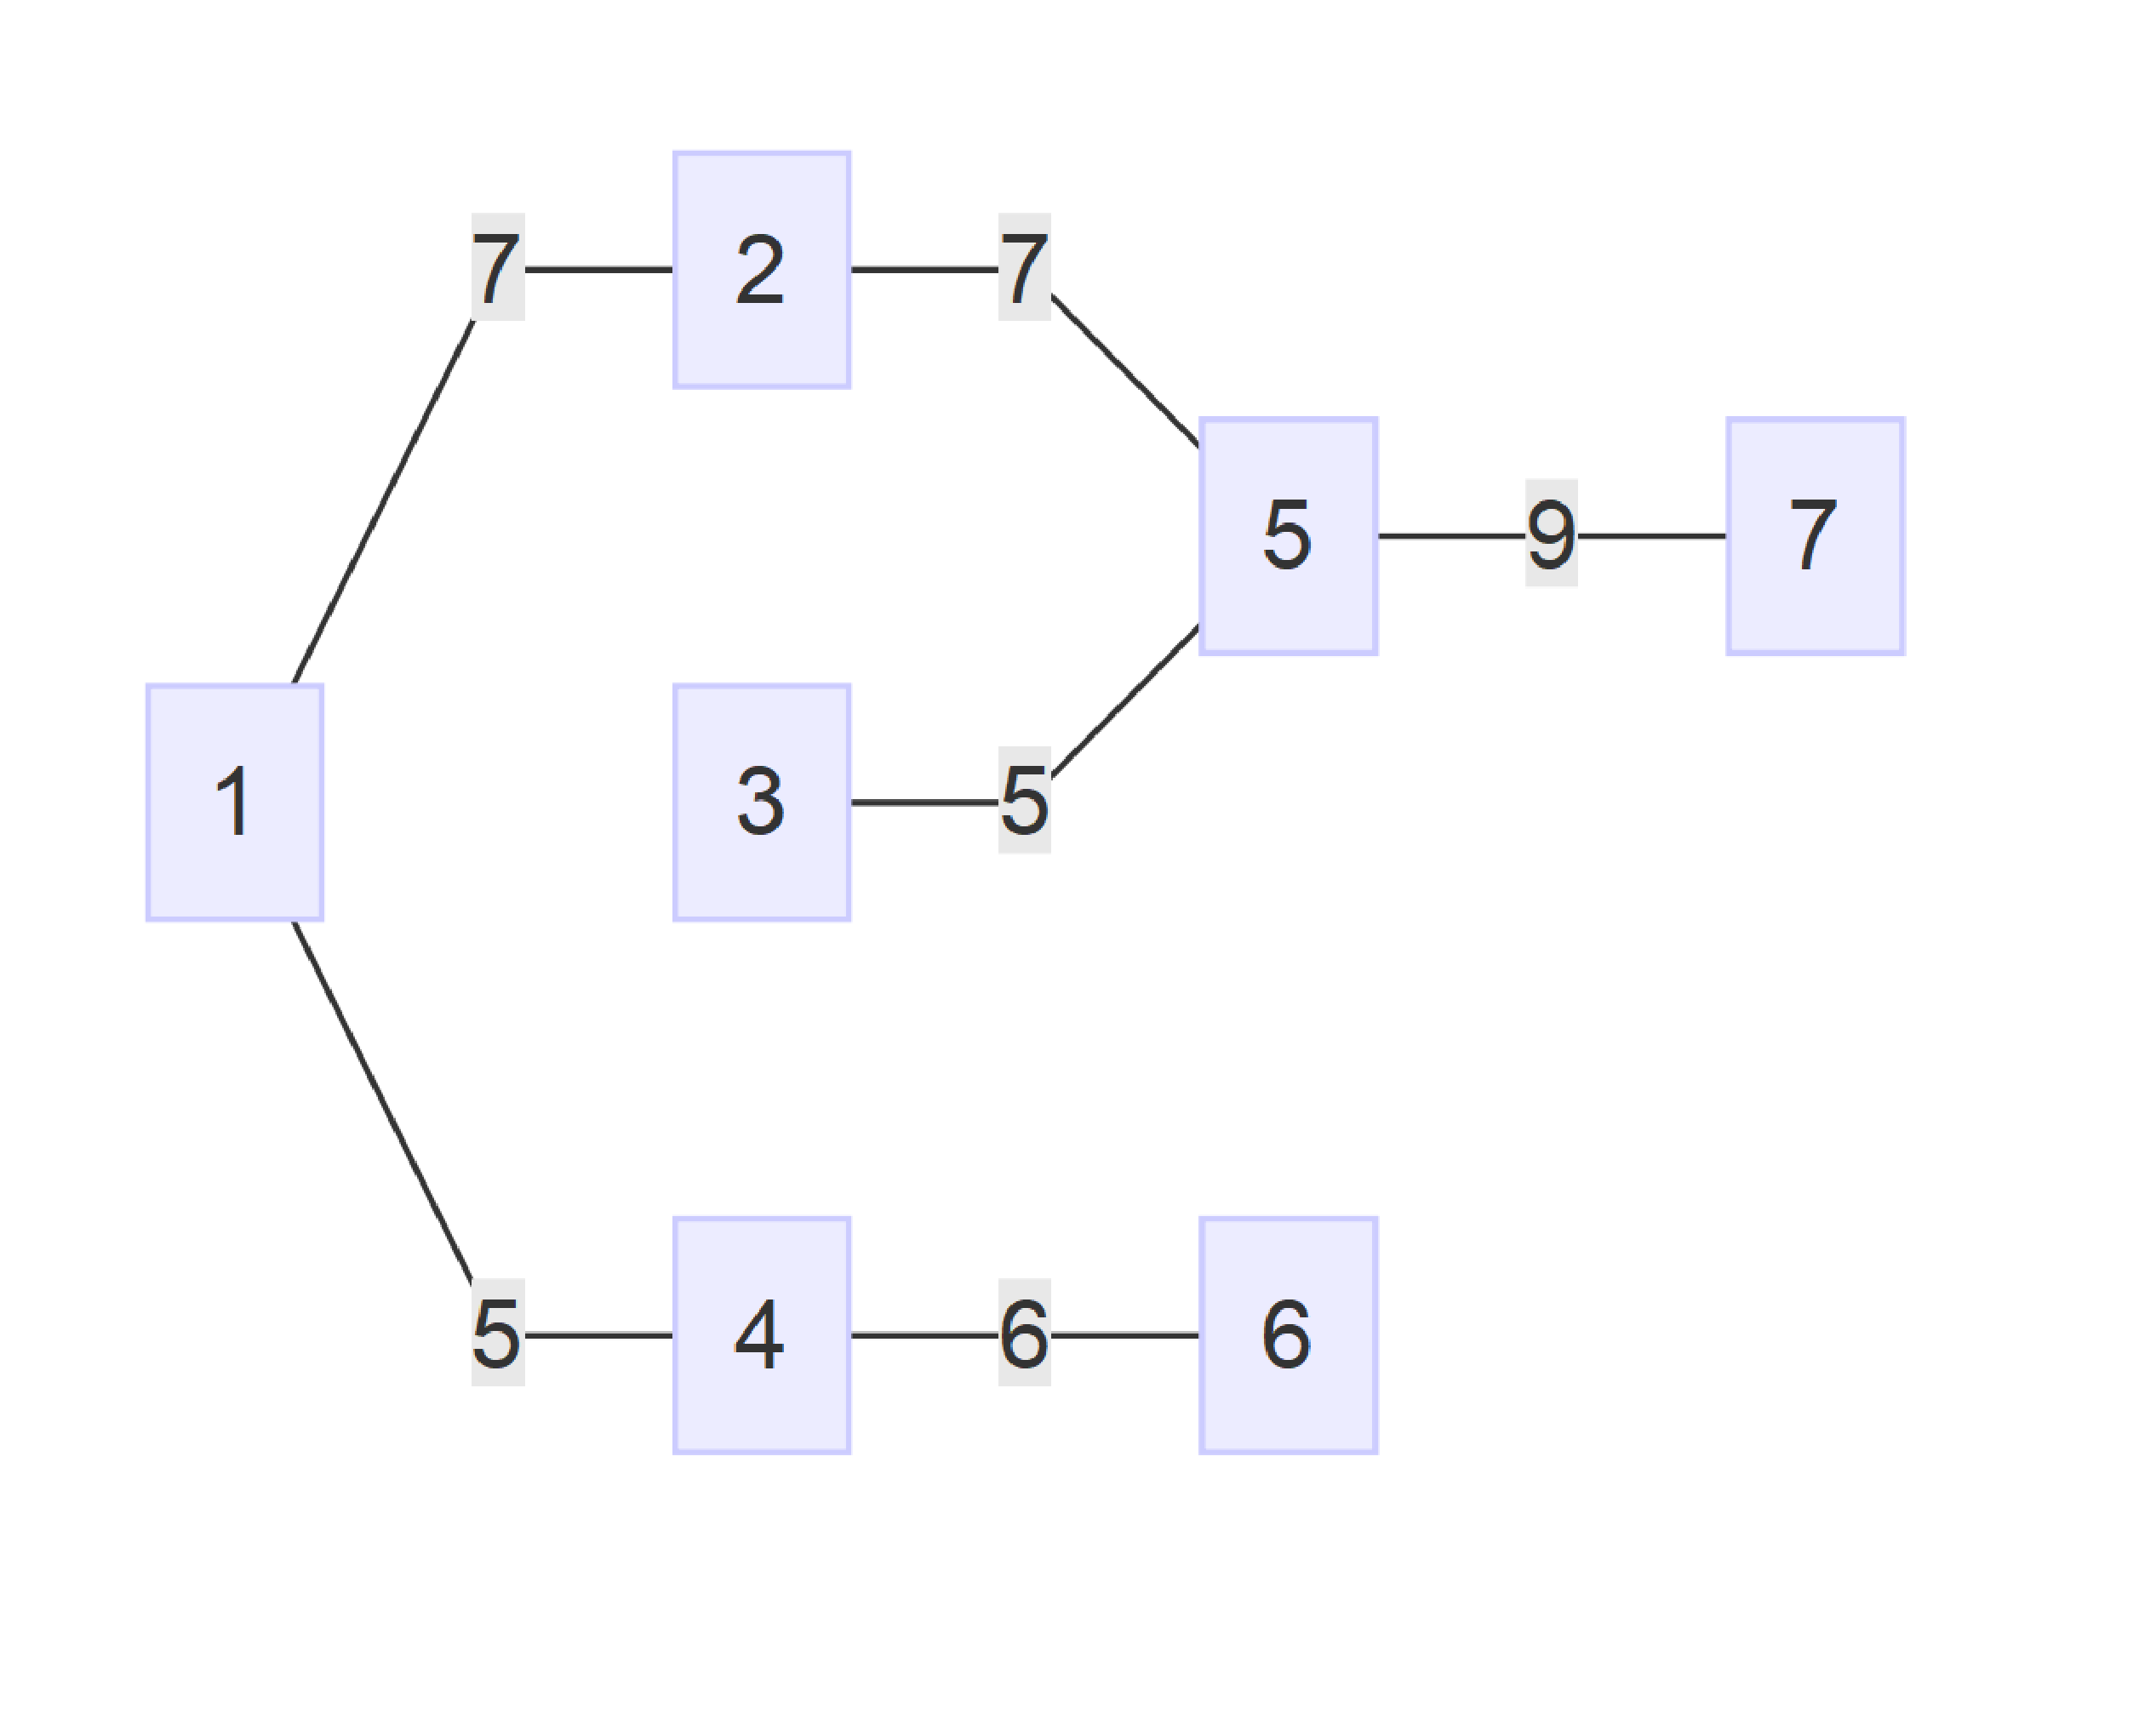
\includegraphics[height=3in]{../Pics/Test-MiniTree-out.eps}

\section{实验分析}
\subsection{效率分析}
\paragraph{$Prim$算法}的时间复杂度取决于数据结构,
使用矩阵则为$O(v^2)$,邻接表为$O(elog_2v)$。
\paragraph{$Kruskal$算法}的时间复杂度$O(elog_2e)$。

\subsection{优化策略}
\paragraph{权值排序优化策略}
将要扫描的结点按其对应弧的权值进行顺序排列,每循环一次即可得到符合条件的结点,大大提高了算法的执行效率。

\subsection{算法比较}
{$Prim$算法}的时间复杂度为$O(v^2)$或者$O(elog_2v)$,只和顶点的数目有关。
而{$Kruskal$算法}的时间复杂度$O(elog_2e)$,只和边的数目有关。
由此可见,$Kruskal$算法适用于边稀疏的情形,而$Prim$算法适用于边稠密的情形。

\newpage
\appendix
\part{附录}
\section{带权图实现}
\begin{lstlisting}[language={C}]
//
// WeightGraph.h
// Created by Along on 2017/5/13.
//

#ifndef GRAPH_WEIGHTGRAPH_H
#define GRAPH_WEIGHTGRAPH_H

// 不可达时的返回值
#define INFINITY (65535)

// 图的定义
typedef struct w_graph *WGraph;

// 创建一个图
WGraph w_graph_create(int n);

// 删除一个图
void w_graph_destroy(WGraph);

// 添加一条边
void w_graph_add_edge(WGraph, int source, int sink, int weight);

// 顶点的数目
int w_graph_vector_count(WGraph);

// 边的数目
int w_graph_edge_count(WGraph);

// 顶点的度
int w_graph_out_degree(WGraph, int source);

// 两个顶点是否邻接
int w_graph_has_edge(WGraph, int source, int sink);

// 边的权
int w_graph_weight_edge(WGraph, int source, int sink);

// 提供遍历数据的接口
void w_graph_foreach(WGraph g, int source,
    void (*f)(WGraph, int src, int sink, int weight, void *),
    void *data);

#endif //GRAPH_WEIGHTGRAPH_H
\end{lstlisting}
\begin{lstlisting}[language={C}]
//
// WeightGraph.c
// 图的封装
// Created by Along on 2017/5/13.
// https://github.com/AlongWY/Graph
//

#include <stdio.h>
#include <stdlib.h>
#include <assert.h>
#include "WeightGraph.h"

//基础带权图定义
//使用可变数组表示的临接矩阵


typedef struct _list {
    int vec;            //临接顶点
    int weight;         //权
} link_list;

struct w_graph {
    int n;                      //顶点个数
    int m;                      //边个数
    struct successors {
        int d;                  //临接点个数
        int len;                //最大临接点个数
        char is_sorted;         //
        link_list list[1];              //临接列表
    } *v_list[1];
};


//创建一个顶点从0 ~ n-1的带权图
WGraph w_graph_create(int n) {
    WGraph g;
    int i;

    g = malloc(sizeof(struct w_graph) +
    sizeof(struct successors *) * (n - 1));
    assert(g);

    g->n = n;
    g->m = 0;

    for (i = 0; i != n; i++) {
        g->v_list[i] = malloc(sizeof(struct successors));
        assert(g->v_list[i]);
        g->v_list[i]->d = 0;
        g->v_list[i]->len = 1;
        g->v_list[i]->is_sorted = 1;
    }

    return g;
}

//释放内存
void w_graph_destroy(WGraph g) {
    int i;

    for (i = 0; i != g->n; i++) {
        free(g->v_list[i]);
    };
    free(g);
}

//添加边和权
void w_graph_add_edge(WGraph g, int u, int v, int weight) {
    assert(u >= 0);
    assert(u < g->n);
    assert(v >= 0);
    assert(v < g->n);

    //是否需要增长list
    while (g->v_list[u]->d >= g->v_list[u]->len) {
        g->v_list[u]->len *= 2;
        g->v_list[u] =
                realloc(g->v_list[u], sizeof(struct successors) +
                 sizeof(link_list) * (g->v_list[u]->len - 1));
    }

    //添加新临接点
    g->v_list[u]->list[g->v_list[u]->d].vec = v;
    g->v_list[u]->list[g->v_list[u]->d].weight = weight;

    g->v_list[u]->d++;

    g->v_list[u]->is_sorted = 0;

    //边数+1
    g->m++;
}

//返回顶点个数
int w_graph_vector_count(WGraph g) {
    return g->n;
}

//返回边个数
int w_graph_edge_count(WGraph g) {
    return g->m;
}

//返回顶点的度
int w_graph_out_degree(WGraph g, int source) {
    assert(source >= 0);
    assert(source < g->n);

    return g->v_list[source]->d;
}

//是否需要进行二分搜索和排序
#define BSEARCH_THRESHOLD (10)

static int list_cmp(const void *a, const void *b) {
    return ((const link_list *) a)->
    vec - ((const link_list *) b)->vec;
}

//二者之间有边则返回1
int w_graph_has_edge(WGraph g, int source, int sink) {
    int i;

    assert(source >= 0);
    assert(source < g->n);
    assert(sink >= 0);
    assert(sink < g->n);

    if (w_graph_out_degree(g, source) >= BSEARCH_THRESHOLD) {
        //确保已经被排序
        if (!g->v_list[source]->is_sorted) {
            qsort(g->v_list[source]->list,
                  g->v_list[source]->d,
                  sizeof(link_list),
                  list_cmp);
        }
        //使用二分查找
        link_list to_find;
        to_find.vec = sink;
        to_find.weight = 0;

        return bsearch(&to_find,
                       g->v_list[source]->list,
                       g->v_list[source]->d,
                       sizeof(link_list),
                       list_cmp) != 0;
    } else {
        //数据量很少,直接遍历
        int vec_degree = g->v_list[source]->d;
        for (i = 0; i != vec_degree; i++) {
            if (g->v_list[source]->list[i].vec == sink) {
                return 1;
            }
        }
    }
    return 0;
}

//返回权
int w_graph_weight_edge(WGraph g, int source, int sink) {
    int i;

    assert(source >= 0);
    assert(source < g->n);
    assert(sink >= 0);
    assert(sink < g->n);

    if (w_graph_out_degree(g, source) >= BSEARCH_THRESHOLD) {
        //确保已经被排序
        if (!g->v_list[source]->is_sorted) {
            qsort(g->v_list[source]->list,
                  g->v_list[source]->d,
                  sizeof(link_list),
                  list_cmp);
        }
        //使用二分查找
        link_list to_find;
        to_find.vec = sink;
        to_find.weight = 0;
        link_list *res = bsearch(&to_find,
                                 g->v_list[source]->list,
                                 g->v_list[source]->d,
                                 sizeof(link_list),
                                 list_cmp);
        return res->weight;
    } else {
        //数据量很少,直接遍历
        for (i = 0; i != g->v_list[source]->d; i++) {
            if (g->v_list[source]->list[i].vec == sink) {
                int res = g->v_list[source]->list[i].weight;
                return res;
            }
        }
        return INFINITY;
    }
}

//提供数据 遍历接口
void w_graph_foreach(WGraph g, int source,
void (*f)(WGraph, int, int, int, void *), void *data) {
    int i;

    assert(source >= 0);
    assert(source < g->n);

    for (i = 0; i != g->v_list[source]->d; ++i) {
        f(g, source, g->v_list[source]->list[i].vec,
         g->v_list[source]->list[i].weight, data);
    }
}
\end{lstlisting}
\section{最小生成树}
\begin{lstlisting}[language={C}]
//
// Graph_tools.h
// Created by Along on 2017/5/13.
//

#ifndef GRAPH_GRAPH_TOOLS_H
#define GRAPH_GRAPH_TOOLS_H

#include "WeightGraph.h"

// tools
// 将图打印出来
void w_graph_show(WGraph);

// 将图成Graphviz的格式输出文件以便于生成图片
void w_graph_show_dot(WGraph, char path[]);

// 封装:由于是无权图, 一次添加二条边
void w_graph_add_edge2(WGraph, int source, int sink, int weight);

// 求最小生成树
// Prim算法
WGraph Prim(WGraph, int start);

// Kruskal算法(其中用到了堆)
WGraph Kruskal(WGraph);

#endif //GRAPH_GRAPH_TOOLS_H
\end{lstlisting}
\begin{lstlisting}[language={C}]
//
// Graph_tools.c
// Created by Along on 2017/5/13.
// https://github.com/AlongWY/Graph
//

#include <stddef.h>
#include <assert.h>
#include <malloc.h>
#include <stdio.h>
#include "WeightGraph.h"
#include "Graph_tools.h"
#include "Binaryheap.h" //堆的实现

//辅助工具
//边遍历工具
struct need_data {
    int *near;
    int *Len;
    int *S;
};

static void update_edge(WGraph g, int src, int sink
                            , int weight, void *data) {
    assert(g);
    if (!((struct need_data *) data)->S[sink]) {
        if (weight < ((struct need_data *) data)->Len[sink]) {
            ((struct need_data *) data)->Len[sink] = weight;
            ((struct need_data *) data)->near[sink] = src;
        }
    }
}

WGraph Prim(WGraph g, int start) {
    int i, j;
    int vec_num = w_graph_vector_count(g);
    WGraph res = w_graph_create(vec_num);
    assert(res);
    assert(start >= 0);
    assert(start < vec_num);

    struct need_data Data;
    Data.S = calloc((size_t) vec_num, sizeof(int));//逐步增加的新顶点集
    Data.Len = calloc((size_t) vec_num, sizeof(int));   //到树的最小边
    Data.near = calloc((size_t) vec_num, sizeof(int));  //最近临接顶点
    for (i = 0; i != vec_num; ++i)
        Data.Len[i] = INFINITY;
    Data.S[start] = 1;
    Data.Len[start] = 0;
    int curr = start;

    for (i = 1; i != vec_num; ++i) {
        //通过curr更新各边最短值
        w_graph_foreach(g, curr, update_edge, &Data);
        int near_len = INFINITY;
        for (j = 0; j != vec_num; ++j) {
            if (!Data.S[j] && Data.Len[j] < near_len) {
                near_len = Data.Len[j];
                curr = j;
            }
        }
        Data.S[curr] = 1;
        w_graph_add_edge2(res, curr, Data.near[curr], Data.Len[curr]);
    }
    free(Data.near);
    free(Data.Len);
    free(Data.S);
    return res;
}

// 存入堆的数据类型
typedef struct _Edge {
    int from;
    int to;
    int len;
} Edge;

// 比较边的大小
int edge_cmp(const void *a, const void *b) {
    return ((Edge *) a)->len - ((Edge *) b)->len;
}

// 初始时将各边插入堆中
static void insertEdge(WGraph g, int src, int sink, 
                            int weight, void *heap) {
    assert(g);
    Edge *edge = malloc(sizeof(Edge));
    edge->from = src;
    edge->to = sink;
    edge->len = weight;
    Heap_insert((BinaryHeap) heap, edge, edge_cmp);
}

//并查集+堆优化Kruskal算法
WGraph Kruskal(WGraph g) {
    int i, SetType;
    int vec_num = w_graph_vector_count(g);
    WGraph res = w_graph_create(vec_num);
    BinaryHeap heap = Heap_create((size_t) w_graph_edge_count(g));
    int *S = calloc((size_t) vec_num, sizeof(int));
    assert(S);

    for (i = 0; i != vec_num; ++i) {
        w_graph_foreach(g, i, insertEdge, heap);
        S[i] = i;                                       //森林
    }
    Edge *e = NULL;

    while (w_graph_vector_count(res) != (w_graph_edge_count(res) / 2 + 1))
    {
        e = Heap_delete_key(heap, edge_cmp);
        //如果加入这条边不会形成圈
        if (S[e->from] != S[e->to]) {
            //接收此边并合并
            w_graph_add_edge2(res, e->from, e->to, e->len);
            SetType = S[e->to];
            for (i = 0; i != vec_num; ++i) {
                if (S[i] == SetType)
                    S[i] = S[e->from];
            }
        }
        free(e);
    }
    Heap_delete(heap);
    return res;
}

\end{lstlisting}

\section{堆的实现}
\begin{lstlisting}[language={C}]
//
// Binaryheap.h
// 堆的简单实现
// Created by Along on 2017/5/14.
//

#ifndef GRAPH_BINARYHEAP_H
#define GRAPH_BINARYHEAP_H

// 堆的定义
typedef struct BinaryHeap *BinaryHeap;

// 创建一个堆
BinaryHeap Heap_create(size_t n);

// 堆的数据量
int Heap_size(BinaryHeap);

// 插入数据
void Heap_insert(BinaryHeap, void *key, 
                int (*cmp)(const void *a, const void *b));

// 删除并取出堆顶元素
void *Heap_delete_key(BinaryHeap, 
                int (*cmp)(const void *a, const void *b));

// 删除堆
void Heap_delete(BinaryHeap);

#endif //GRAPH_BINARYHEAP_H
\end{lstlisting}

\begin{lstlisting}[language={C}]
//
// Binaryheap.c
// Created by Along on 2017/5/14.
//

#include <stddef.h>
#include <malloc.h>
#include <assert.h>
#include "Binaryheap.h"

// 堆的数据结构
struct BinaryHeap {
    int n;
    int len;
    void *data[1];
};

// 创建堆
BinaryHeap Heap_create(size_t n) {
    BinaryHeap h = malloc(n * sizeof(BinaryHeap) +
                         sizeof(void *) * (n - 1));
    assert(h);
    h->n = 0;
    h->len = (int) n;
    return h;
}

//插入数据
void Heap_insert(BinaryHeap h, void *key, int (*cmp)
                                (const void *, const void *)) {
    assert(key);
    //动态扩展堆大小
    if (h->n >= h->len) {
        h->len *= 2;
        h = realloc(h, sizeof(BinaryHeap) + sizeof(void *) * (h->len - 1));
    }

    //上滤
    int hole = ++h->n;
    void *copy = key;

    h->data[0] = copy;
    for (; cmp(key, h->data[hole / 2]) < 0; hole /= 2) {
        h->data[hole] = h->data[hole / 2];
    }
    h->data[hole] = h->data[0];
    h->data[0] = NULL;
}

// 元素上滤,保证堆的平衡
static void percolateDown(BinaryHeap h, int hole, 
        int (*cmp)(const void *, const void *)) {
    int child;
    void *tmp = h->data[hole];
    for (; hole * 2 <= h->n; hole = child) {
        child = hole * 2;
        if (child != h->n && cmp(h->data[child + 1], h->data[child]) < 0)
            ++child;
        if (cmp(h->data[child], tmp) < 0)
            h->data[hole] = h->data[child];
        else
            break;
    }
    h->data[hole] = tmp;
}

// // 删除并取出堆顶元素
void *Heap_delete_key(BinaryHeap h, int (*cmp)
                        (const void *, const void *)) {
    assert(h->n > 0);
    void *res = h->data[1];

    h->data[1] = h->data[h->n--];
    percolateDown(h, 1, cmp);
    return res;
}

// 堆的数据量
int Heap_size(BinaryHeap h) {
    return h->n;
}

// 删除堆
void Heap_delete(BinaryHeap h) {
    free(h);
}
\end{lstlisting}
\end{document} 